% acmtr.tex
% revised 1/20/97
% $Header: acmtr.tex,v 1.5 2/14/96 11:07:57 boyland Exp $

\documentclass[hyperref]{acmtrans2e}
\usepackage{url}
\usepackage{graphicx}
\usepackage{wrapfig}




\graphicspath{ {./images/} }
%&t&{\tt #}&
%&v&\verb|#|&

\newcommand{\BibTeX}{{\rm B\kern-.05em{\sc i\kern-.025em b}\kern-.08em
    T\kern-.1667em\lower.7ex\hbox{E}\kern-.125emX}}

\firstfoot{Detection of cats in images, DTU, June 2015}

\runningfoot{Detection of cats in images, DTU, June 2015}

\markboth{Anna Maria Walach}{Detection of cats in images}

\title{Detection of cats in images}
\author{ANNA MARIA WALACH (s121540) \\Technical University of Denmark\\02238 Biometric Systems}
\begin{abstract}
The \LaTeX\ {\tt acmtrans} document style formats articles in 
the style of the ACM transactions.  Users who have prepared their
document with \LaTeX\ can, with very little effort, produce
camera-ready copy for these journals.  
%Then the ACM production department
%will re-typeset from scratch anyway, introducing typographical errors.
\end{abstract}

\category{D.2.7}{Software Engineering}{Distribution and Main\-ten\-ance}%
[documentation]

\category{H.4.0}{Information Systems Applications}{General}


\terms{Algorithms, Experimentation}

\keywords{cat, detection, images}

\begin{document}

\setcounter{page}{111}

\maketitle

\section{Introduction}
There are more and more projects that uses live streaming and social media power to help and safe feral cats. Some of them are meant to control the population in the area \cite{LAPS:2015}, other focus on raising awareness about feral cats, spaying and neutering importance \cite{TinyKittens:2015} or just to increase changes of finding a new home for homeless cats and kittens \cite{CritterRoom:2015}.

\begin{wrapfigure}[13]{r}{0.5\textwidth}
\centering
    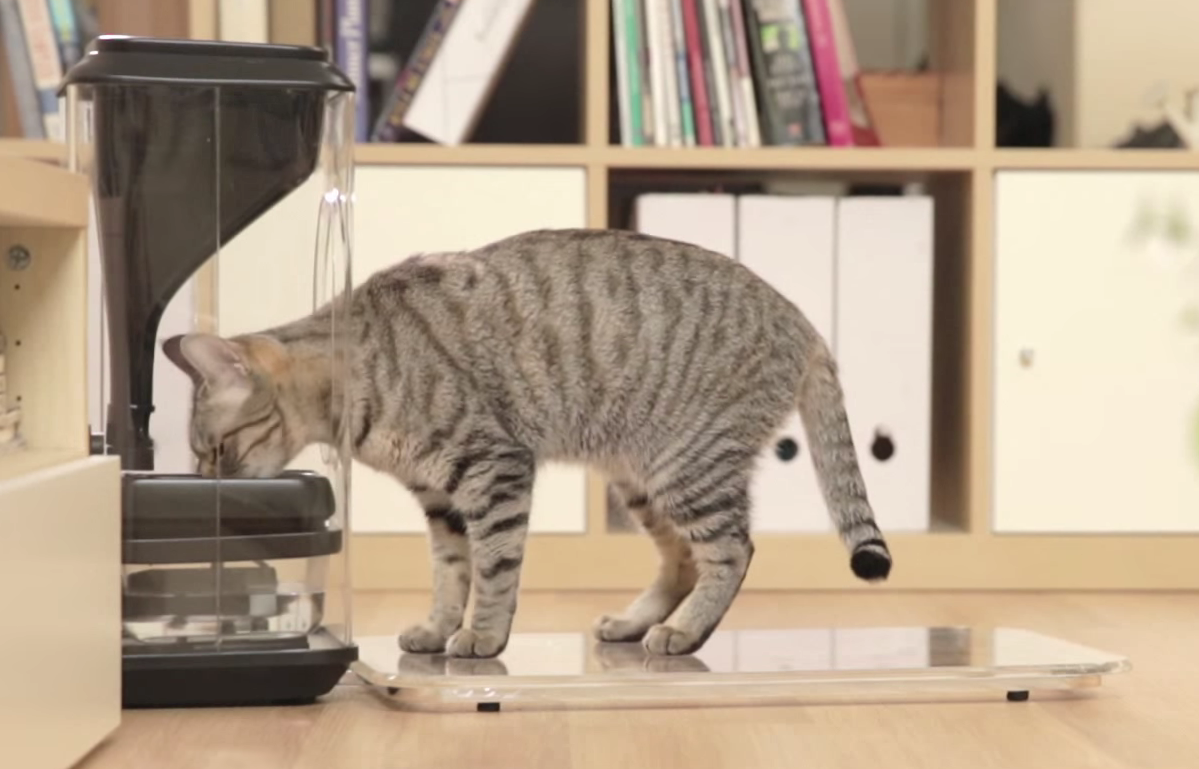
\includegraphics[width=0.48\textwidth]{bistro}
  \caption{CatFi product used by a cat.}
  \label{fig:bistro}
\end{wrapfigure}
People are also more interested in health and safety of their own pets. Lower prices of video technologies and smarthone popularity helped to create various apps for controlling your pet lifestyle. \cite{CatFi:2015} created an automatic feeder with cat identification system and connected it to the smartphone app (product can be seen in fig. \ref{fig:bistro}. It allows owner to supervise the amount of dry food and water his cats are consuming everyday, to receive alarms in case of abnormalities and even spy on them while eating. 

The PiP \cite{PiP:2013} app is designated to help people find their lost cats and dogs. According to American Human Society, almost 3.5 million pets are lost each year and about 80\% of dogs and 98\% of cats are never re-united with their families. The authors of the smarthone app allows the owners to made profiles for their pets (including pictures) and in case the pet is missing, you launch the "alarm" on that pet, together with last seen location. If anyone finds a homeless animal, he may send the photo of it to the PiP app, which automatically try to match one of the lost pets with found pet. 

Increasing number of pets' photographies also encouraged camera producers to implement appropriate support for it in their devices. Right now, Fujifilm company introduced Auto Dog / Cat Detection function \cite{FujiFilm:2009} in some of their cameras that allows to automatically detect pet's face on the image and put auto-focus on it. 
 
\subsection{Problem description}
Almost all of the applications and initiatives described in previous section already use or would benefit from the cats detection and/or identification. In this research I would like to focus on topic of cat detection in images. The main interest is on the use case of detecting cats presence in shots from live cameras and streams. Such images are characterized by  diversified, often bad lighting settings, with possible presence of another animals or human beings. I will perform a state-of-the-art survey and then perform a comparison of existing, available algorithms. 

\section{The state of the art}
Reliable comparison of existing software for detecting cats in pictures is hard to performed. It is caused by a few factors:
\begin{itemize}
\item~\textbf{black-box algorithms} - many algorithms, that claim to have high accuracy, are part of the hardware product \cite{CatFi:2015} or closed-source app \cite{PiP:2013}. This way it is impossible to make a theoretical comparison of the algorithms and usually significantly hampers possibility of performing experiments with test data, as the products' interfaces are not adjusted to bulk operations. 
\item~\textbf{high diversity of use cases} - although there are a lot of studies focusing on cat face detection, usually the classification or testing environmental does not check robustness of the algorithm in typical real-time scenarios. The classification is e.g. made as cat vs still life \cite{features:2007,edges:2011} or as cat/dog breed detection \cite{breed:2012}.
\item~\textbf{different test sets} - even for algorithms with similar use cases, e.g. cat vs still life, different test set are in use to estimate the accuracy of algorithm, which makes it significantly harder to perform direct comparisons. Usually articles use their own data sets \cite{breed:2012,features:2007,edges:2011} and only some of them compare to standard data bases, like Pascal 2007 cats database \cite{breed:2012}. 
\end{itemize}

As the main idea of this research is to find an algorithm that will allow for highly accurate detection of cat faces in the pictures, only articles presenting "cat vs still life" classification will be taken under consideration.

\subsection{Unsupervised image categorization}
\label{sec:google}
One of the more interesting approaches to this problem was presented in \cite{google:2012}. Researchers from Google and Stanford university constructed large scale unsupervised learning tool. It was a 9-layered neural network build on a cluster that consisted of 1 000 machines with total of 16 000 cores. The network was trained with 10 million unlabelled images, all of them had the same size and local contrast normalization was applied on them. The model consisted of 1 bilion connections and it took 3 days to train the classifiers. Final results are very promising for overall image categorization issue, because authors claims to have 15.8\% accuracy for ImageNet dataset (22 000 object categories), which is a 70\% improvement in comparison to the previous state of the art. 

However, the most interesting part of \cite{google:2012} for this research is that after performing face-detection experiment, authors tried to used trained classifiers to detect cats. The results are very promising - the random guess had 64.8\% chance, while this algorithm was able to detect cats with 74.8\% accuracy.

This algorithm and use of deep learning networks seems to be a promising technique for classification of images categories, however seemed to be lacking needed accuracy for binary classification (cat vs not-cat). 
\subsection{Pet detection method for digital camera}
\label{sec:camera}

Another interesting project was performed by \cite{edges:2011}. They tried to construct a cat and dogs face detection mechanism for use in camera auto-focus and auto-exposure. They were not satisfied with current method, because camera has a very high constraints about calculation time and power consumption, were most of the studies focus on high recall and small false-detection. 
\begin{wrapfigure}[16]{r}{0.5\textwidth}
\centering
    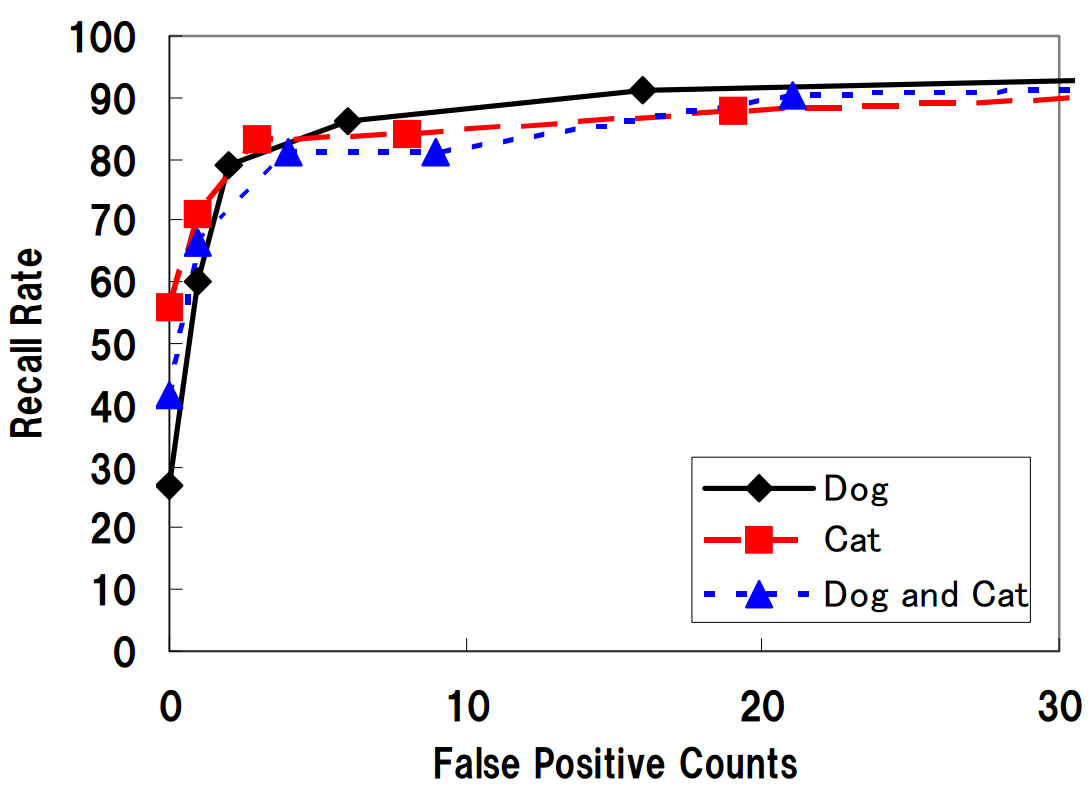
\includegraphics[width=0.48\textwidth]{roc_edges}
  \caption{ROC curves achieved as a result of \protect\cite{edges:2011}.}
  \label{fig:roc_edges}
\end{wrapfigure}
Authors decided to use four direction features as an input for the classifier. In order to speed-up the process, classification of an image window was hierarchical - if coarse classifier did not detect a sign of face in the window, it was automatically rejected and not send to more detailed and feature-rich fine classifier. 

The results are very promising. As described in fig. \ref{fig:roc_edges}, with the average recall on 90\%, the false positive count is around 20. Although the FPC may seem high (the sample size was 400, with 200 of non-animal pictures), it is still on user-acceptable level. What is more important, the processing time was only 245ms on ARM9 device with 166MHz core. It is impressive result, especially because this solution turned out to be also very robust to illumination changes. Authors measured how color and intensity fluctuation caused by illumination changes influence the recall rate. Intensity changes didn't cause the recall rate to drop under 80\% even on very high intensity values. With 50\% color fluctuation recall rate still oscillate between 80\%-90\%. 

Although the results are not perfect (usually recall rate do not exceed 90\%), short processing time allows to use this algorithm in real-time cases, with may be important case with live streaming observation. This solution can be used as a part of pet-identification algorithm, that informs appropriate person when the cat appears in the camera (e.g. if it is known it is pregnant and needs to be caught and checked) and in such cases time is always a crucial value. It could be an interesting experiment to see if a little bit of power efficiency (i.e. better processing unit) could significantly improve the recall rate.

\subsection{Shape and texture features for cat face detection}
\label{sec:demo}
The solution presented in \cite{shape:2008} is the only one with existing available implementation. Also, as part of it, the on-line interface was provide for testing \cite{demo:2013}. Authors of \cite{shape:2008} decided, that both texture and shape are important features of cat face detection. Their solution has two steps - in first, they create separately trained shape and texture detector, both based on Haar-like features. As a second step they are jointly training fusion classifier (joint shape and texture). Both shape and texture classifier were trained on differently normalized data. Their features are based on oriented gradients.

\begin{wrapfigure}[16]{r}{0.5\textwidth}
\centering
    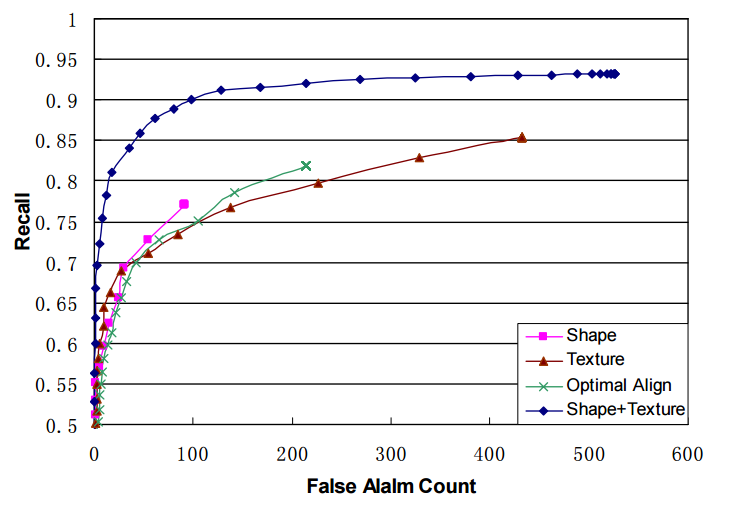
\includegraphics[width=0.48\textwidth]{roc_shape}
  \caption{ROC curves achieved as a result of \protect\cite{shape:2008}.}
  \label{fig:roc_shape}
\end{wrapfigure}
Important part of that study was creating a database of 10 000 annotated cat pictures \cite{base:2008} (annotations of 9 points in the cat face, like ears triangles, nose, mouth). This pictures will be the part of this research dataset.

The results of that study are presented in fig. \ref{fig:roc_shape}. The recall rate oscillate around 90\% with 100 FPC for the joint texture and shape detector. Because huge focus of \cite{shape:2008} was on feature engineering and comparing their features with different standard approaches, authors also made a direct comparison, using Pascal 2007 data set. They claim that Average Precision (AP) of their approach is 0.364, when best reported method has AP equalled to 0.24. 

The study seemed to find interesting and quite straight forward method of detecting cats face. Coming from human face detection, they adjusted their feature choice with respect to differences appearing in cat face and then tested different type of gradient features to picked the most suitable one for this aim. However, it should be noted that this article is 7 years old and probably some of the studies presented in previous sections may have better results, but it is hard to estimate, as everyone are using different databases for testing.

\subsection{Stationary features and cat detection}
In the study \cite{features:2007} authors presents a novel approach based on pose-indexed features. Firstly, the image is processed using custom edge detectors and grey scale histogram. Then, the second level feature is the head-belly pose, described as a reference frame, rotated accordingly to the pose vector. The expected result is a frame containing the cat.

The classifiers used in that project are boosted trees and asymmetric weighting by sampling. The classifiers are are using hierarchical search strategy, to avoid very costly scene processing. By using this methods, authors managed to avoid fragmentation of the data for separate training of pose classifiers. 

\begin{wrapfigure}[14]{r}{0.5\textwidth}
\centering
    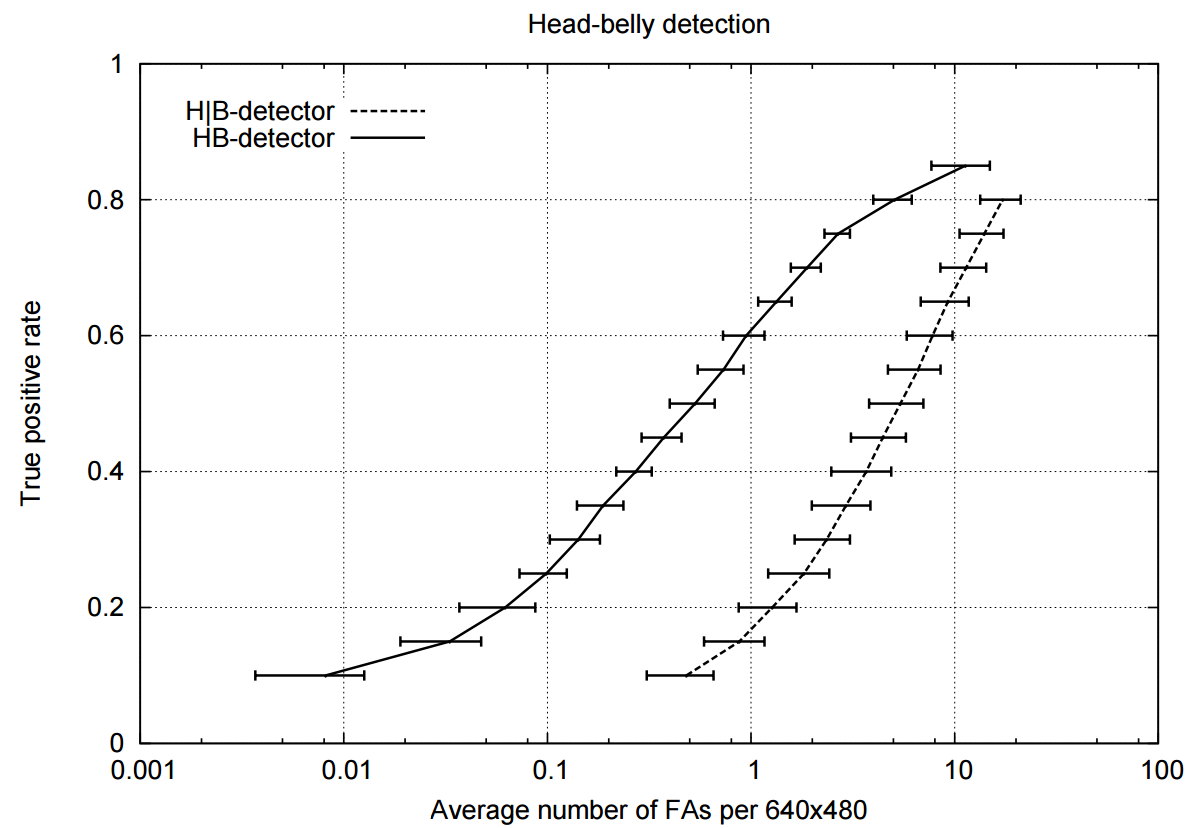
\includegraphics[width=0.48\textwidth]{roc_features}
  \caption{ROC curves achieved as a result of \protect\cite{features:2007}.}
  \label{fig:roc_features}
\end{wrapfigure}

The results of that study for the head-belly detection task are presented in fig. \ref{fig:roc_features}. The recall is around 80\% and 85\% (depending on method), with FAC equalled to respectively 17 and 11 on average with variation 3.5. Authors also performed head detection experiment with a little bit better results (recall 95\% with FAC ranging from 6.65 to 12.31 depending on method).

Summing up, that novel approach seems to be very effective, but the images were mostly focusing on cat and still life cases, so it is hard to estimate the efficiency of this study in e.g. forest live streaming. Also, that study, similar to previous one described, is quite old if we take under consideration how fast machine learning is developing in last years, so it would probably be an interesting project to revise those ideas and try to apply them to modern approaches. 

\subsection{Discussion}

Described articles are presenting different approaches to the same problem, with focus on different factors (accuracy, efficiency, performance). In regards to the main 
\begin{wrapfigure}[25]{r}{0.5\textwidth}
\centering
    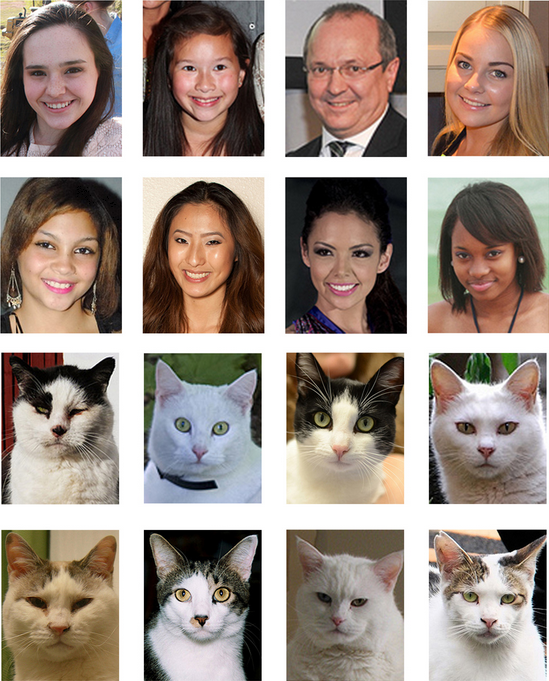
\includegraphics[width=0.48\textwidth]{cat_vs_human}
\centering
  \caption{First two rows - human recognized as cats by \protect\cite{demo:2013}. Last two rows - cats recognized as human by OpenCV face detection algorithm}
  \label{fig:cat_vs_human}
\end{wrapfigure}
problem in this article (cat detection in live streams), probably the study described in section \ref{sec:camera} is the best approach. It is the only study that perform actual experiments focused on illumination invariance. It is hard to estimate robustness of algorithm depending on pose variation, because none of the study actually focus on that. Although everyone are mentioning that cat detection is harder than human detection because of much greater pose possibilities, no tests are performed to check the robustness of algorithm to it.

The main difficulty in comparing various methods of cat face detection is using different databases with different sizes (ranging from 400 to a million) and different non-cat data. From all the studies, only the one described in sec. \ref{sec:google} did have a database containing human faces or other animals. Interesting test was performed by an artists(!) group Shinseungback Kimyonghun \cite{vs:2013}. They used Kittydar \cite{demo:2013}, the application based on algorithm described in sec. \ref{sec:demo} and OpenCV face detection algorithm to parse pictures of humans and cats. They ended up with 200 images, half of them with humans recognized by Kittydar as cats and half of them with cats recognized by OpenCV as humans. Part of their results is shown in figure \ref{fig:cat_vs_human}.

\section{Problem analysis}
This section is meant to describe the properties of algorithm suitable for cat detection. It will be started with recalling of expected algorithm applications:
\begin{itemize}
\item~\textbf{be first part of cat identification system} - as such, it should have low false rejection rate. High false acceptance is allowed, as it would be filtered by identification subsystem.
\item~\textbf{work in poor light settings} - The live stream takes place in different locations - house, forests, gardens, often 24/7, and there may be situation when no artificial light is provided. The algorithm should be as robust as possible to light variance.
\item~\textbf{distinguish between cats and cat-like, humans, other animals} - a lot of current studies does not take under consideration that human faces or other animals may be the part of background. It is important to prepare features so that not too many false acceptance are caused by another beings (although, as mentioned above, false acceptance ratio is not the most important statistic).
\end{itemize}
\subsection{Algorithm properties}
With these applications in mind, one can summarize it with list of algorithm properties:
\begin{itemize}
\item~robust to light/pose variation 
\item~as low as possible false rejection count
\item~false acceptance count may be high
\item~additional focus on distinguishing between cats and other living creatures
\end{itemize}
\subsection{Implementation considerations}
\section{Experiments}
\subsection{Data set}
shape - comparision of different approaches

fujifilm - photo restrictions

it is important that such algorithm is robust to pose variation and illumination level.
\subsection{Proposed method}
\subsubsection{Features}
\subsubsection{Classifier}

\subsection{Bibliography}
\bibliographystyle{acmtrans}
\bibliography{acmtr}
\begin{received}
Received June 2015;
\end{received}

\end{document}





